\section{Problema 1: ZombieLand}

\subsection{Descripci\'on de la problem\'atica}

En un pa\'is con \emph{n} ciudades, se encuentra una determinada cantidad de Zombies y de Soldados por cada una de ellas; donde el problema es exterminar la invasi\'on zombie. Para ello, es necesario un enfrentamiento \textit{zombies vs soldados} por cada ciudad. Para que el combate sea viable en una ciudad, es decir, se logre matar a todos los zombies de la misma, es necesario que la cantidad de zombies sea, a lo sumo, diez veces m\'as grande que la cantidad de soldados.\\

Se sabe de antemano cu\'antos zombies y cu\'antos soldados se encuentran atrincherados en cada ciudad. Los soldados acuartelados no pueden moverse de la ciudad en la que est\'an, pero s\'i se cuenta con una dotaci\'on de soldados extra que se la puede ubicar en cualquiera de las \emph{n} ciudades para salvarlas. La cantidad de soldados extra es ilimitada, mas los recursos para trasladarlos no lo son. El costo del traslado depende de cada ciudad. Siempre que se respete el presupuesto del pa\'is, se pueden trasladar todos los soldados necesarios para salvar a cada ciudad.\\

Debido a que los recursos econ\'omicos son finitos, no siempre va a ser posible salvar a las \emph{n} ciudades. Lo que se desea en este problema es maximizar la cantidad de ciudades salvadas, respetando el presupuesto. Es decir, se deben establecer la cantidad de soldados extra enviados a cada ciudad de modo que la cantidad de ciudades salvadas sea la \'optima (es decir, la máxima) y gastando un monto por debajo o igual al presupuesto.  El algoritmo debe tener una complejidad temporal de $O(n.log(n))$, siendo $n$ la cantidad de ciudades del pa\'is.\\

A continuaci\'on se presenta un ejemplo sobre c\'omo resolver el problema, dado un caso espec\'ifico.\\

Se nos presenta un pa\'is con cuatro ciudades ($A$, $B$, $C$ y $D$), el cual tiene un presupuesto a gastar de 100\$. Las ciudades est\'an caracterizadas de la siguiente manera:


 \begin{figure}[h!]
   \begin{center}
 	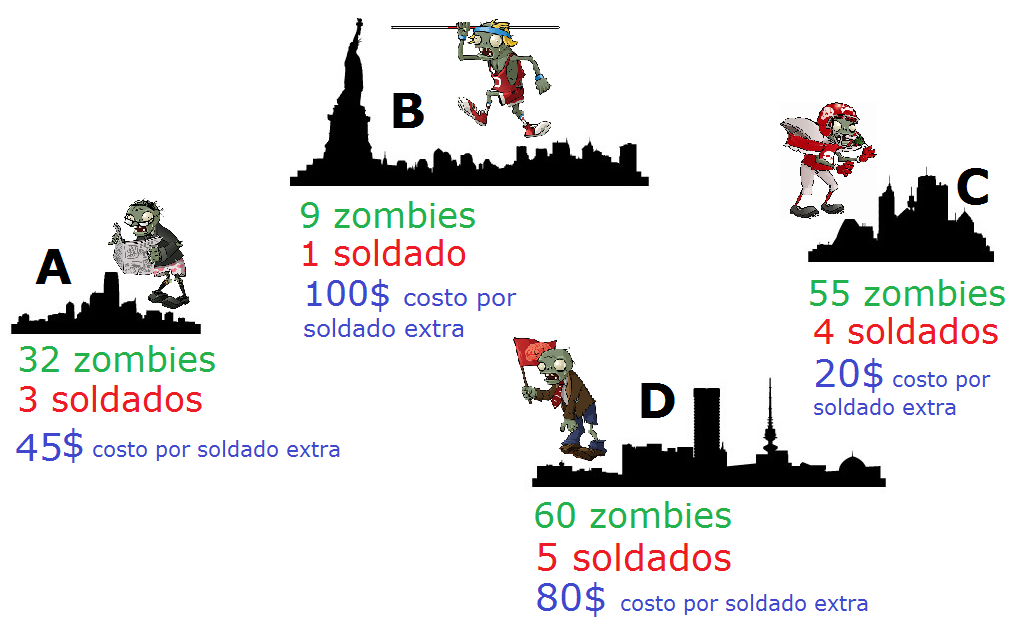
\includegraphics[scale=0.6]{imagenes/ej1/ciudades.png}
 %	\caption{Casillas que \emph{cubre} un caballo}
   \end{center}
 \end{figure} 

\newpage
 En la siguiente tabla se muestran las diferentes elecciones que se pueden realizar al contratar soldados extra, teniendo en cuenta el presupuesto inicial, indicando cu\'antas ciudades son salvadas.

\begin{table}[htb]
\centering
\begin{tabular}[c]{|l|l|l|l|l|l|l|}

		\hline
		Casos &\multicolumn{4}{|c|}{Cantidad de Soldados}& Presupuesto Gastado & Ciudades salvadas\\
		&\multicolumn{4}{|c|}{extra por ciudad}& &  \\
		\cline{2-5}
		&  $A$  &  $B$  &  $C$  &  $D$  & & \\
		\hline
		Caso 1& 1 & 0 & 0 & 0 & 45\$ & A y B \\
		\hline
	    Caso 2& 2 & 0 & 0 & 0 & 90\$ & A y B \\
		\hline
		Caso 3& 1 & 0 & 1 & 0 & 65\$ & A y B \\
		\hline
		\textbf{Caso 4}& \textbf{1} &\textbf{ 0} & \textbf{2} & \textbf{0} & \textbf{85\$} & \textbf{A, B y C} \\
		\hline
		Caso 5& 0 & 1 & 0 & 0 & 100\$ & B \\
		\hline		
		Caso 6& 0 & 0 & 1 & 0 & 20\$ & B \\
		\hline
		Caso 7& 0 & 0 & 2 & 0 & 40\$ & B y C \\
		\hline
		Caso 8& 0 & 0 & 1 & 1 & 100\$ & B y D \\
		\hline
		Caso 9& 0 & 0 & 0 & 1 & 80\$ & B y D \\
		\hline
		Caso 10& 0 & 0 & 0 & 0 & 0\$ & B \\
		\hline
		
	\end{tabular}
%\caption{Tabla muy sencilla.}
%\label{tabla:sencilla2}
\end{table}

Se puede observar que la ciudad $B$ siempre se encuentra en el conjunto de Ciudades Salvadas, esto se debe a que al momento de ser ingresada la cantidad de zombies es menor (o igual) a diez veces la cantidad de soldados. 

En este ejemplo, la soluci\'on buscada (la \'optima) es la del \emph{Caso 4}, si bien esta no es la que menor presupuesto gasta, es la que logra salvar la mayor cantidad de ciudades (3).

\newpage
\subsection{Resoluci\'on propuesta y justificaci\'on}

Para la resoluci\'on del problema decidimos utilizar un algoritmo goloso, que salvar\'a en cada paso a la ciudad que m\'as le convenga en ese momento, es decir, la que permita maximar la cantidad de ciudades salvadas.\\

Como primera instancia, el algoritmo simplemente calcula, para cada ciudad, cu\'anto ser\'ia el costo de salvarla. Para ello, primero se calcula la cantidad de soldados extra necesarios y luego se multiplica por el costo de traslado de cada unidad:\\


	\begin{codesnippet}
	\begin{verbatim}
		soldados_extras_necesarios = redondeo_hacia_arriba((zombies - (soldados_existentes * 10)) /10)
		
		costo_total = costo_unitario * soldados_extras_necesarios
	\end{verbatim}
	\end{codesnippet}

Luego de haber obtenido una magnitud con la cual se pueden comparar las ciudades entre s\'i, se ordenan las ciudades de menor a mayor en base al costo de salvarla, para ser recorridas secuencialmente y enviar los ej\'ercitos requeridos hasta que se agote el presupuesto.\\

Notar que si alguna ciudad no requiere soldados extras para ser salvada, entonces ser\'an las primeras en ser salvadas, dado que \texttt{costo_total} ser\'a igual a 0.\\
 
Se recorren secuencialmente las ciudades ordenadas por \texttt{costo_total}, de modo que para cada una se va a comparar el costo de salvarla contra el presupuesto restante en ese momento\\ (\texttt{presupuesto_actual}). Si es factible salvar la ciudad, se resta \texttt{costo_total} de \texttt{presupuesto_actual} y se env\'ian las tropas necesarias a la ciudad; en caso contrario se la marca como ciudad perdida.\\

Vale aclarar que el orden impuesto a las ciudades implica que cuando ya no se pueda salvar a una ciudad, no se podr\'a salvar a ninguna otra de las restantes.\\
 
%Como en este vector las ciudades no aparecen en orden creciente por su n\'umero, debemos reordenarlas. Debido a que el \emph{id} de cada ciudad va a ser \'unico y va a encontrarse en el intervalo [0, n-1], se lo recorre secuencialmente colocando cada ciudad en la posici\'on de su \textit{id} dentro de un nuevo vector \emph{respuesta} . \textcolor{red}{Ver que este parrafo me aprece que no quedo muy claro...} \textcolor{blue}{es necesario este p\'arrafo? habla del stdout... no me parece necesario en absoluto... yo lo sacar\'ia}\\

A continuación demostraremos que el algoritmo resuelve efectivamente el problema planteado.\\

\textbf{Teorema}
El algoritmo resuelve el problema planteado, salvando la mayor cantidad de ciudades posibles.\\

\textbf{Demostraci\'on}
Para demostrar el teorema enunciado, supondremos que nuestro algoritmo no devuelve una solución óptima, y tomaremos la solución óptima con más ciudades salvadas en común.
Sean $C_{k}$ las ciudades de la solución óptima y $D_{k}$ las ciudades de la solución dada por el algoritmo, y supondremos que están ordenadas de menor a mayor, según el costo de ser salvadas.
Sea $C_{j}$ la primer ciudad distinta a las ciudades de $D$, de modo que $C_{i}$ = $D_{i}$ $\forall i, i < j$.\\

Entonces, hasta $C_{i-1}$, el costo total por salvar dichas ciudades es el mismo al de $D$ hasta $D_{i-1}$. Pero ya que el algoritmo elige siempre la ciudad que (pudiendo salvarse) cueste lo menor posible, eso significa que $C_{i}$ tiene un costo igual o mayor al de $D_{i}$, con lo cual si en $C$ reemplazamos $C_{i}$ por $D_{i}$, seguimos teniendo presupuesto (en particular, mayor que el que se tenía) y se salvan la misma cantidad de ciudades, por lo que debe ser óptimo.\\

Pero esta nueva solución, es una solución óptima que tiene más ciudades en común que $C$, por lo que es absurdo, ya que $C$ era la solución óptima que más ciudades en común tenía con $D$.\\

El absurdo proviene de suponer que $D$ no es óptimo y que por lo tanto la solución óptima con más ciudades salvadas en común con $D$, no es $D$.\\

Así, $D$ debe ser óptimo, en el sentido de que debe tener la mayor cantidad ciudades que pueden ser salvadas, para el presupuesto y costos para cada ciudad dados.

\newpage
\subsection{An\'alisis de la complejidad}
La complejidad de nuestra soluci\'on es $O(n.log(n))$, siendo \emph{n} la cantidad de ciudades del pa\'is.\\

En primera instancia, guardamos los datos de las ciudades pasadas por $stdin$ en $structs$ y los dejamos dentro de un vector, para luego poder utilizarlas de un modo pr\'actico. Como esto se realiza secuencialmente, tiene costo lineal \textbf{\textit{O(n)}}.

\begin{algorithm}[h!]
\caption{zombieland}
\For{\emph{each} ciudad $\in$ pa\'is}{
	Calcular la cantidad de soldados extra necesarios y el costo de salvarla.\\
	Almacenar esta informaci\'on en un vector \emph{datos} mediante \textit{push_back()}
}
Ordena al vector \emph{datos} mediante \textit{sort()}\\
\While{pueda salvar}{
	\If{puede ser salvada}{
		Indicar cantidad de soldados extras enviados y actualizar el \texttt{presupuesto_actual}
	}
}
\While{haya ciudades insalvables}{
	cantidad de soldados extras enviados = 0
}
%\textcolor{blue}{es necesario este cacho? habla del stdout... no me parece necesario en absoluto... yo lo sacar\'ia}\\
%\For{\emph{each} ciudad \emph{en vector} datos}{
%	Insertar en el vector \emph{respuesta}[ciudad.id] la ciudad actual. 
%}
\end{algorithm}
%\textcolor{red}{En el codigo, yo pondria este reordenamiento dentro de zombieland, ya que hay que considerarlo para medir tiempos.}\\
%\textcolor{blue}{A mi no me parece que sea necesario para medir tiempos... o sea, arrancar de la instancia pasada por parametro, salvo que la limemos y usemos avls, heaps, etc. no me parece necesario contarlas. lo mismo para escribir, la respuesta est\'a, en el ej2 tenemos que calcular un pedazo de respuesta post algoritmo y lo hacemos y lo consideramos, el std out extra porque deber\'iamos considerarlo? es algo que nos piden para visualizar, si las cosas andan mal, porque pueden llegar a estar mal}\\

%\textcolor{red}{Dijo el ayudante que eso si habia que ponerlo....}

El c\'odigo presenta un \textbf{primer ciclo \emph{for}} que calcula el costo de salvar a cada ciudad y las agrega mediante push_back() a un vector. El ciclo recorre linealmente todas las ciudades por lo que tiene complejidad $O(n)$. 

El c\'alculo de salvar a cada ciudad coincide con el descripto en la secci\'on anterior, el cual, por ser operaciones aritm\'eticas, es $O(1)$. Armar el nuevo \emph{struct} para insertar dentro del vector \emph{datos} tambi\'en posee un costo constante $O(1)$. La funci\'on \href{http://www.cplusplus.com/reference/vector/vector/push_back/}{push\_back()} \footnote{http://www.cplusplus.com/reference/vector/vector/push_back/} tiene costo $O(1)$ amortizado, lo que implica que cuando no precisa redimensionar el vector cuesta esto, y cuando lo hace, toma tiempo lineal en la cantidad de elementos. Como insertamos durante todo el ciclo tomamos el costo amortizado $O(1)$.
Por lo tanto, la complejidad total del primer ciclo for nos da \textbf{\textit{O(n)}}.\\

Le sigue \textbf{ordenar el vector} con estos datos, para ello usamos \href{http://www.cplusplus.com/reference/algorithm/sort/}{sort()} \footnote{http://www.cplusplus.com/reference/algorithm/sort/} cuya complejidad es \textbf{\textit{O(n.log(n)})}.\\

A continuaci\'on, se realizan dos \textbf{\'ultimo ciclos \emph{while}} el primero salva todas las ciudades que pueda, mientras dure el presupuesto y el segundo deja en \emph{0 soldados enviados} a las ciudades que no pueden ser salvadas. Estos c\'alculos aritm\'eticos y asignaciones son todos de complejidad constante $O(1)$. El primer ciclo toma $O(ciudades\_salvadas)$ y el segundo $O(n-ciudades\_salvadas)$ dando como resultado un recorrido lineal sobre todas las ciudades, por lo tanto lo hace con complejidad \textbf{\textit{O(n)}}.\\

%\textcolor{blue}{Para mi no va...}\textcolor{red}{Dijo que siiiiii}\\

%Finalmente, se debe \textbf{reordenar el vector} obtenido hasta ahora para que quede en orden creciente respecto de su \textit{id}. Como esto se hace recorriendo secuencialmente el primer vector, asign\'andole uno a uno los elementos al nuevo vector \emph{respuesta} indexados; s\'olo hace una pasada lineal con costo \textbf{\textit{O(n)}}.\\

Como cada paso de los mencionados son secuenciales, las complejidades se suman, obteniendo:\\

$O(n)$ + $O(n.log(n))$ + $O(n)$ 
% + $O(n)$
 que es igual a \textit{\textbf{O(n.log(n))}} por propiedades de $O$.


\newpage

\subsection{C\'odigo fuente}

	\begin{codesnippet}
	\begin{verbatim}
struct ciudad{
    int zombies;
    int soldados;
    int costo;
};
	\end{verbatim}
	\end{codesnippet}

	\begin{codesnippet}
	\begin{verbatim}
struct ciudad2{
    int numCiudad;
    int soldadosNecesarios;
    int costoTotal;
    bool operator< (const ciudad2& otro) const{
        return costoTotal < otro.costoTotal;
    }
};
	\end{verbatim}
	\end{codesnippet}


	\begin{codesnippet}
	\begin{verbatim}
int main(int argc, char const *argv[]){
    chrono::time_point<chrono::system_clock> start, end;
    long int cantCiudades, presupuesto;
    vector<ciudad> pais;
//Leemos informacion del problema
    cin >> cantCiudades;
    cin >> presupuesto;
    for (int i = 0; i < cantCiudades; ++i){
        ciudad alguna;
        cin >> alguna.zombies;
        cin >> alguna.soldados;
        cin >> alguna.costo;
        pais.push_back(alguna);
    }
    long int salvadas = 0;
    start = chrono::system_clock::now();
//Aplicamos el algoritmo
    vector<ciudad2> res = zombieland(cantCiudades, presupuesto, pais, salvadas);
    end = chrono::system_clock::now();
    vector<long int> entregados(cantCiudades);
//Stdout pedido
    for (int i = 0; i < cantCiudades; ++i){
        entregados[res[i].numCiudad] = res[i].soldadosNecesarios;
    }
    cout << salvadas << " ";
    for (int i = 0; i < cantCiudades; ++i){
        cout << entregados[i] << " ";
    }
    cout << endl;
    chrono::duration<double> elapsed_seconds = end-start;
    cout << "Tiempo: " << elapsed_seconds.count() << endl;
    return 0;
}
	\end{verbatim}
	\end{codesnippet}
	
	
	\begin{codesnippet}
	\begin{verbatim}
const vector<ciudad2> zombieland(long int cantCiudades, long int presupuesto, 
const vector<ciudad>& pais, long int& salvadas){
    salvadas = 0;
    vector<ciudad2> datos;
    for (int i = 0; i < cantCiudades; ++i){
        ciudad2 actual;
//ID de la ciudad
        actual.numCiudad = i;
//Calculamos el costo de salvar la ciudad i
        double diferencia = (pais[i].zombies - pais[i].soldados * 10);
        if (diferencia > 0)
            actual.soldadosNecesarios = ceil(diferencia/10);
        else
            actual.soldadosNecesarios = 0;
        actual.costoTotal = actual.soldadosNecesarios * pais[i].costo;
//Lo agregamos al vector
        datos.push_back(actual);
    }
//Ordenamos el vector de menor a mayor costo para salvarlas
    sort(datos.begin(), datos.end());
    long int dif = presupuesto;
//Vemos cuantas salvamos respetando el presupuesto
    int i = 0;
    while(i<cantCiudades && dif >= 0){
        dif = presupuesto - datos[i].costoTotal;
        if (dif>=0){
            salvadas++;
            presupuesto = dif;
            ++i;
        }
    }
//Las que sobran no se salvan
//seteamos los soldados necesarios en 0 para imprimir una respuesta correcta
    while(i<cantCiudades){
        datos[i].soldadosNecesarios = 0;
        ++i;
    }
    return datos;
}
	\end{verbatim}
	\end{codesnippet}
\newpage
\subsection{Experimentaci\'on}

\subsubsection{Constrastaci\'on emp\'irica de la complejidad}


\subsubsection{Experimentaci\'on variando s\'olo el par\'ametro n}

Para realizar la contrastaci\'on emp\'irica de la complejidad de nuestro algoritmo, decidimos comenzar con un muestreo aleatorio de ciudades y presupuestos, aumentando la cantidad de ciudades en cada prueba.

La siguiente tabla indica cu\'anto tiempo utiliz\'o el algoritmo para resolver el problema, siendo $n$ la cantidad de ciudades en cada caso.

\begin{table}[htb]
\centering
\begin{tabular}[c]{|l|l|}

		\hline
n & Tiempo en segundos\\
		\hline
1000	&	0.0002860962\\
		\hline
2000	&	0.0006116975\\
		\hline
3000	&	0.0009399667\\
		\hline
4000	&	0.0010920646\\
		\hline
5000	&	0.0015213336\\
		\hline
6000	&	0.0020432861\\
		\hline
7000	&	0.0024080363\\
		\hline
8000	&	0.0027960707\\
		\hline
9000	&	0.0032532473\\
		\hline
10000	&	0.0036220356\\
		\hline
		
	\end{tabular}
%\caption{Tabla muy sencilla.}
%\label{tabla:sencilla2}
\end{table}

El gr\'afico resultante fue el siguiente:

 \begin{figure}[h!]
   \begin{center}
 	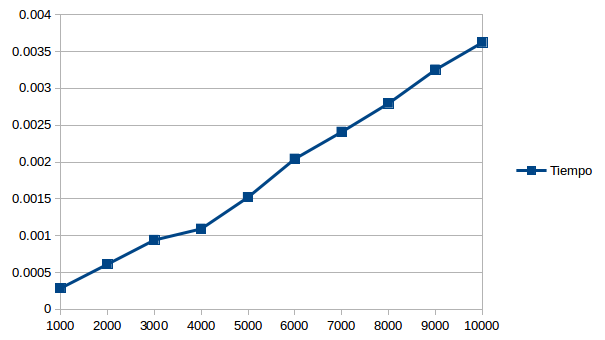
\includegraphics[scale=0.8]{imagenes/ej1/Mediciones/Grafico1.png}
% 	\caption{}
% 	\label{caballito}	
   \end{center}
 \end{figure}

De acuerdo al an\'alisis de este gr\'afico, podemos ver que aparenta ser una curva con poca inclinaci\'on, similar al gr\'afico de $O( n.log(n) )$, que fue la complejidad propuesta.\\

Para una mejor interpretaci\'on del muestreo obtenido, se realiz\'o una linealizaci\'on, dividiendo los tiempos por $log(n)$. De este modo, si la curva del gr\'afico resultante es una recta indicar\'ia que emp\'iricamente demuestra ser un algoritmo de complejidad $O(n.log(n))$.

\newpage

 \begin{figure}[h!]
   \begin{center}
 	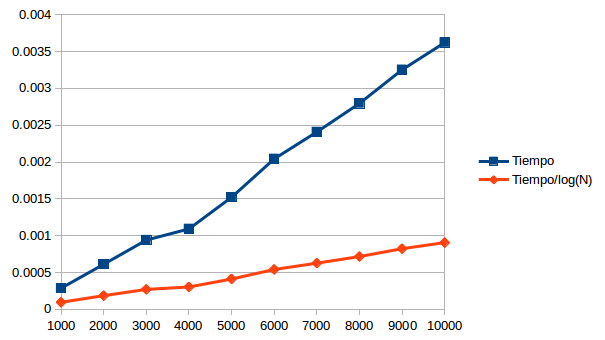
\includegraphics[scale=0.8]{imagenes/ej1/Mediciones/Grafico2.png}
% 	\caption{}
% 	\label{caballito}	
   \end{center}
 \end{figure}

 En esta comparaci\'on, podemos ver que al dividir la curva inicial por $log(n)$, se obtiene pr\'acticamente una funci\'on lineal. Esto nos indica que se condice emp\'iricamente con la hip\'otesis de Complejidad $O(n.log(n))$ (Cota de Complejidad Te\'orica).\\
 
 \newpage
\subsubsection{Experimentaci\'on variando el par\'ametro n y el presupuesto asociado} 
 
Luego realizamos una nueva prueba, para mostrar que el algoritmo solamente depende de la cantidad de ciudades, sin importar cu\'al sea el presupuesto asociado. Como en todos los casos vamos a realizar el $sort()$, que tiene complejidad $O(n.log(n))$, el gr\'afico deber\'ia ser similar.\\

%\textcolor{red}{Aca habria que poner de cuanto es el presupuesto en cada caso, porque sino queda como algo indefinido ''presupuesto grande'' o ''presupuesto chico''}

Primero analizamos los tiempos de ejecuci\'on de nuestro algoritmo para distintas ciudades aleatorias con un presupuesto para todas de $1.000.000.000$\$.
 \begin{figure}[h!]
   \begin{center}
 	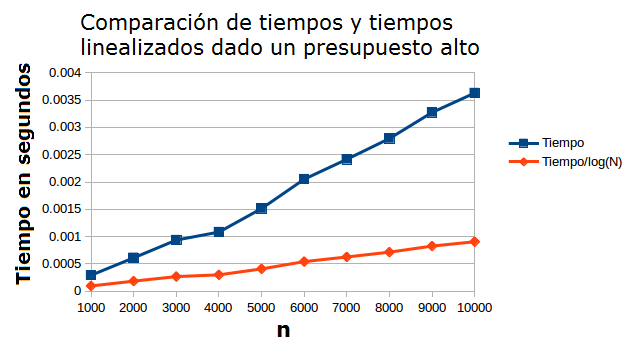
\includegraphics[scale=0.8]{imagenes/ej1/Mediciones/Grafico3.png}
% 	\caption{}
% 	\label{caballito}	
   \end{center}
 \end{figure}


 A continuaci\'on, analizamos los tiempos de ejecuci\'on de las mismas ciudades aleatorias del caso anterior pero asignandoles a todas un presupuesto de $10$\$.
  \begin{figure}[h!]
   \begin{center}
 	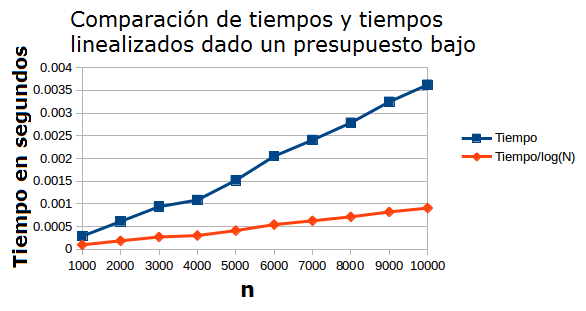
\includegraphics[scale=0.9]{imagenes/ej1/Mediciones/Grafico4.png}
% 	\caption{}
% 	\label{caballito}	
   \end{center}
 \end{figure}
 
 \newpage
Efectivamente, utilizando tanto presupuestos altos como bajos, la curva presenta un comportamiento similar.

Si comparamos las tablas de valores para ambos casos, podemos ver que los tiempos no difieren notablemente. Adem\'as, podemos ver c\'omo oscilan entre s\'i los tiempos de cada caso acorde avanza el n.\\

\begin{table}[htb]
\centering
\begin{tabular}[c]{|l|l|l|l|l|}



		\hline
		n &\multicolumn{2}{|c|}{Presupuesto Alto}& \multicolumn{2}{|c|}{Presupuesto Bajo}\\
		\cline{2-5}
		& Tiempo & Tiempo/log(n) & Tiempo & Tiempo/log(n)\\
		\hline
	1000 & 0,0002944123	& 9,81374406666668E-005 & 0,0002878731 & 9,59577063333334E-005 \\
	\hline
	2000 &	0,0006123812 &	0,0001855121 & 	0,0006116416 & 	0,0001852881 \\
	\hline	
	3000 & 0,0009376308	& 0,0002696572	& 	0,0009373774 & 	0,0002695843 \\
	\hline
	4000 & 0,0010842365 & 0,0003010046	& 	0,0010840265 & 	0,0003009463 \\
	\hline
	5000 & 	0,0015145134 & 0,0004094419	& 	0,0015181007 & 	0,0004104117 \\
	\hline
	6000 & 	0,0020518541 &	0,0005430842 & 	0,0020493215 & 	0,0005424138 \\
	\hline
	7000 & 0,0024156113	&	0,0006282314 & 	0,0024062528 & 	0,0006257975 \\
	\hline
	8000 & 0,0027960219	&	0,0007163611 & 	0,0027869656 & 	0,0007140408 \\
	\hline
	9000 & 0,0032732535	&	0,0008277827 & 	0,0032490964 & 	0,0008216735 \\
	\hline 
	10000 & 0,0036292888 &	0,0009073222 & 	0,0036244519 & 	0,000906113 \\
	\hline

		
	\end{tabular}
%\caption{Tabla muy sencilla.}
%\label{tabla:sencilla2}
\end{table}

En nuestra experimentaci\'on se puede notar que la variaci\'on de los tiempos de ejecuci\'on s\'olo depende de la cantidad de ciudades (\emph{n}) y no del presupuesto que cuente cada una.



\newpage
 